% ------------------------------------------------------------
\begin{figure}[t]
    \centering
    \vspace{2mm}
    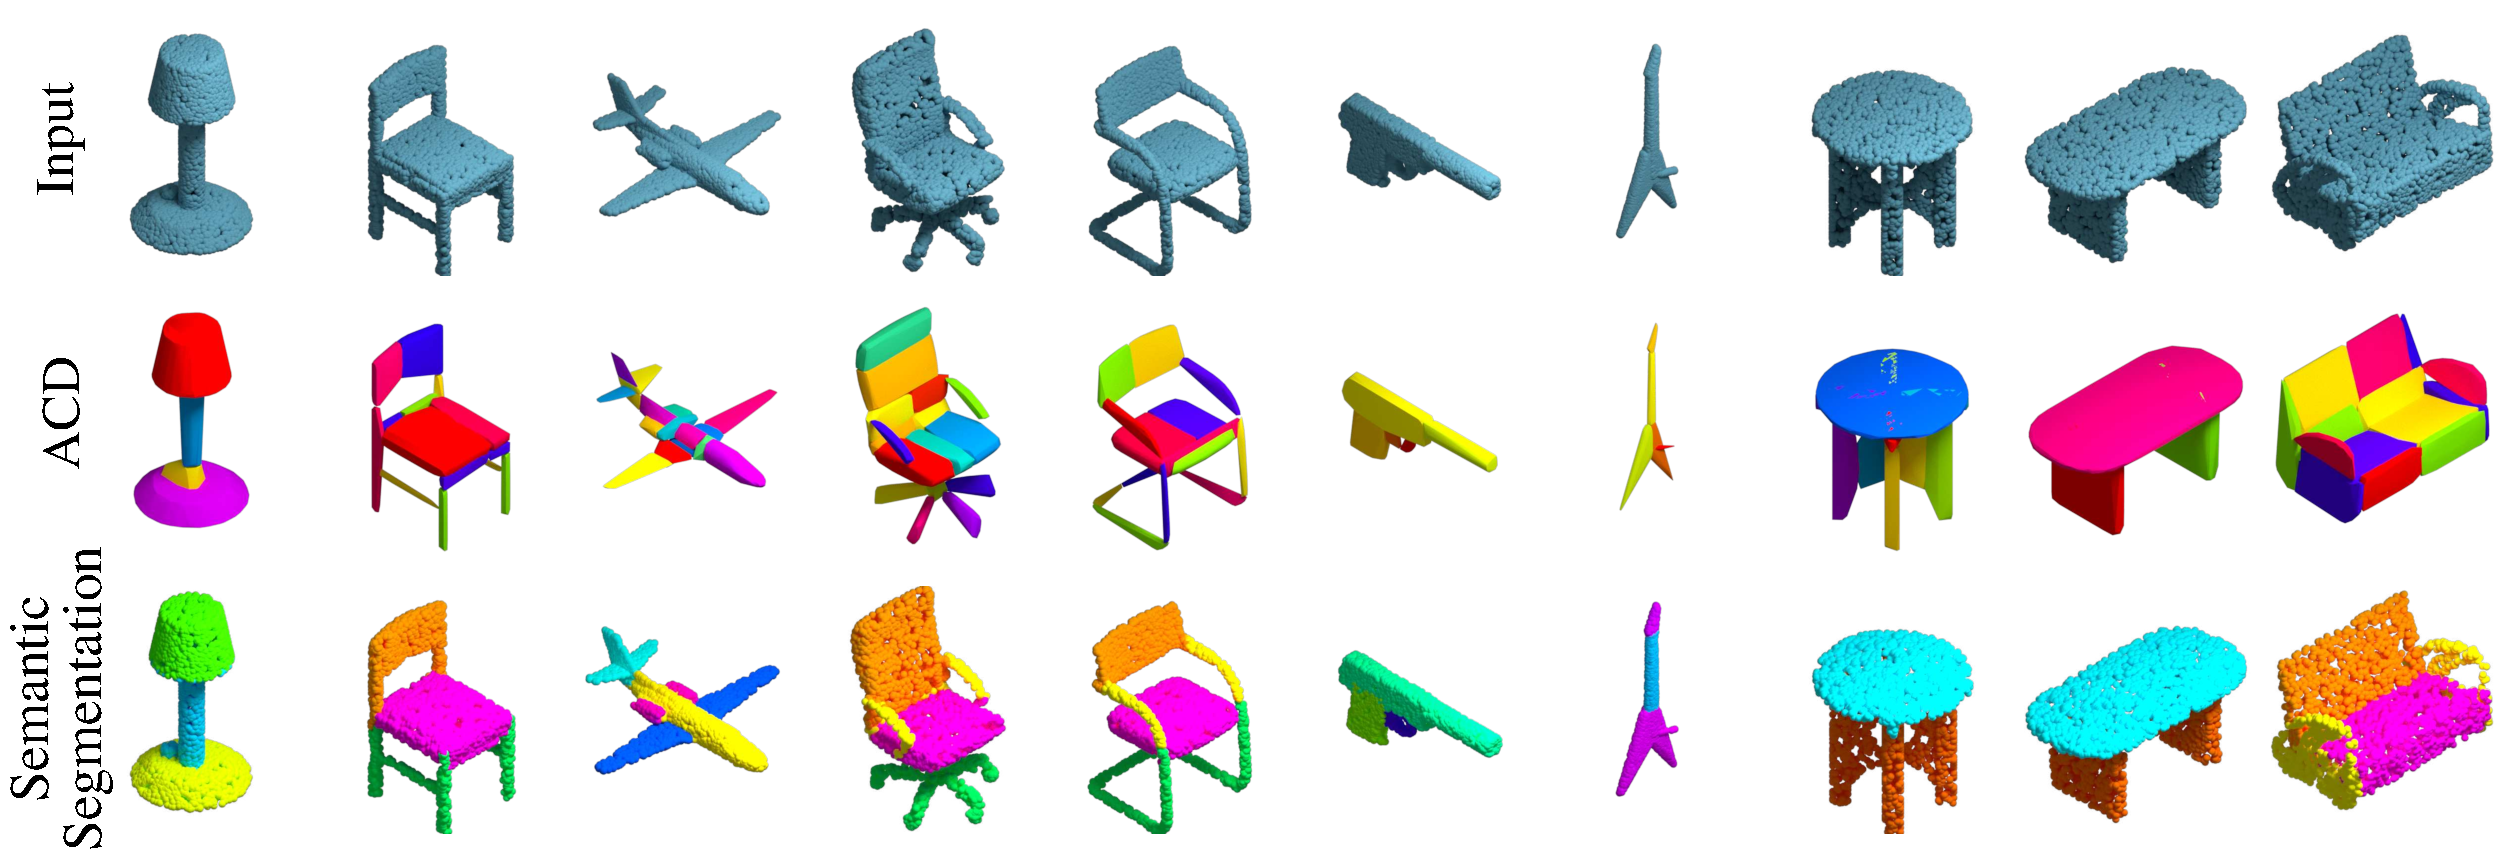
\includegraphics[width=\linewidth]{acd/imgs/acdexamples.pdf}
    \vspace{2mm}
    \caption{ \small{
    Input point clouds (first row), convex components \emph{automatically} computed by ACD (second row) and
    \emph{human-labeled} point clouds (last row) from the ShapeNet~\cite{Chang2015ShapeNetAI} part segmentation benchmark.
    Note -- \textit{\textbf{(i)}} different colors for the ACD components only signify different parts-- no semantic
    meaning or inter-shape correspondence is inferred by this procedure; 
    \textit{\textbf{(ii)}} for the human labels, colors do convey semantic meaning: \eg the backs of chairs are always orange;
    \textit{\textbf{(iii)}} while the ACD decompositions tend to oversegment the shapes, they contain 
    most of the boundaries present in the human annotations, 
    suggesting that the model has similar criteria for decomposing objects into subparts;
    \eg chair's legs are separated from the seat,
    wings and engines are separated from the airplane boundary, pistol trigger is separated from the rest, \etc~
    }}
    \label{fig:samples-of-acds}
\end{figure}



% ------------------------------------------------------------
\subsection{Approximate Convex Decomposition}
\label{sec:acd}
In this subsection, we provide an overview of the shape decomposition approach used to 
generate the training data for our self-supervised task.
A detailed description of the method used in this work can be found in~\cite{vhacd}.

Decomposing complex shapes as sets of convex components is a well studied problem~\cite{acd,vhacd,acanalysis,minimumncd}.
Given a polyhedron $P$, the goal is to compute the smallest set of convex polyhedra $\mathcal{C} = \{C_k | k=1,...,N\}$, 
such that the union $\cup_{k=1}^{k=N}C_i$ corresponds to $P$.
However, exact convex decomposition of polyhedra is an NP-Hard problem~\cite{ecd} and 
leads to decompositions containing too many components, rendering it impractical for use
in most applications (ours included).
This can be circumvented by Approximate Convex Decomposition (ACD) techniques.
ACD relaxes the convexity constraint of exact convex decomposition by allowing every
component to be \emph{approximately convex} up to a concavity $\epsilon$.
The way concavity is computed and how the components are split varies according to different 
methods~\cite{vhacd,fastacd,acd,acanalysis,minimumncd}.
In this work, we use an approach called Volumetric Hierarchical Approximate Convex Decomposition (V-HACD)~\cite{vhacd}.
The reasons for utilizing this approach are threefold.
First, as the name suggests, V-HACD performs computations using volumetric representations, which can be easily
computed from dense point cloud data or meshes and lead to good results
without having to resort to costly decimation and remeshing procedures.
Second, the procedure is reasonably fast and can be applied to open surfaces of arbitrary genus.
Third, V-HACD guarantees that no two components overlap, which means that there is no
part of the surface that is approximated by more than one component.
In the next paragraph, we describe V-HACD in detail.

\vspace{2mm}
\noindent{\textbf{V-HACD.}} Since the method operates on volumetric representations,
the first step is to convert a shape into an occupancy grid.
If the shape is represented as a point cloud, one can compute an occupancy grid by
selecting which cells are occupied by the points and filling its interior.
In our case, since our training shapes are from ShapeNet~\cite{Chang2015ShapeNetAI} which come with meshes, we chose to compute the occupancy grid by voxelizing the meshes using~\cite{voxelizer}.
Once the voxelization is computed, the algorithm proceeds on computing convex components by
recursively splitting the volume into two parts.
First, the volume is centered and aligned in the coordinate system according to its principal
axis.
Then, one of the three axis aligned planes is selected as a splitting plane that
separates the volume in two different parts.
This procedure is applied multiple times until we reach the maximum number of desired components
or the concavity tolerance is reached.
The concavity $\eta(\mathcal{C})$ of a set of components $\mathcal{C}$ is computed as follows:
\begin{equation}
\eta(\mathcal{C}) = \max_{k=1,...N}d(C_k, CH(C_k))
\end{equation}
where $d(X,Y)$ is the difference between the volumes $X$ and $Y$;
$CH(X)$ is the convex hull of $X$;
and $C_k$ is the $k$th element of the set $\mathcal{C}$.
The splitting plane selection happens by choosing one of the axis aligned planes which minimizes an energy $E(K, \mathbf{p})$,
where $K$ is the volume we are aiming to split and $\mathbf{p}$ is the splitting plane.
This energy is defined as:
\begin{equation}
    E(K, \mathbf{p}) = E_{con}(K, \mathbf{p}) + \alpha E_{bal}(K, \mathbf{p}) + \beta E_{sym}(K, \mathbf{p}),
\end{equation}
where $E_{con}$ is the connectivity component, which measures the sum of the normalized concavities between both sides of volume;
$E_{bal}$ is the balance component, which measures the dissimilarity between both sides;
and $E_{sym}$ is the symmetry component, which penalizes planes that are orthogonal to a potential revolution axis.
$\alpha$ and $\beta$ are weights for the last two terms.
In all our experiments we used the default values of $\alpha = \beta = 0.05$.
We refer the reader to~\cite{vhacd} for a detailed description of the components in the energy term.

\vspace{2mm}
\noindent{\textbf{Assigning component labels to point clouds.}} 
The output of ACD for every shape is a set of convex components represented by convex meshes.
For each shape, we sample points on the original ShapeNet mesh and on the mesh of every ACD component.
We then propagate component labels to every point in the original point cloud by using
nearest neighbor matching with points in the decomposition. 
%
More precisely, given an unlabeled point cloud $\{ p_i \}_{i=1}^{N}$, this assigns a component 
label $\Gamma(p_i, \mathcal{C})$ to each point $p_i$ via

\begin{equation}
    \Gamma(p_i, \mathcal{C}) = \argmin_{k = 1 \dots |\mathcal{C}|} \bigg[ \min_{p_j \in C_k} || p_i - p_j ||  \bigg].
\end{equation}



%% ------------------------------------------------------------
%\begin{figure}[t]
%    \centering
%    % \includegraphics[width=\linewidth]{ecdcomp.pdf}
%    % \framebox(\textwidth,90pt){}
%    \emptybox{90pt}
%    \caption{Comparison between exact (second row) and approximate convex decomposition (bottom row).
%    Exact convex decomposition (second row) always yields convex components, perfectly preserving the
%    original shape (top row).
%    However, this method tends to produce a big number of components, making it unpractical for
%    most applications.
%    % \arc{Why not take a \textit{single} shape, and do multiple values of $\epsilon$ of ACD - exact decomposition on the left, all the way to large approximation on the right-most? [figure with one row]}
%    }
%    
%    \label{fig:ecdcomp}
%\end{figure}




% ------------------------------------------------------------
\subsection{Self-supervision with ACD}
 The component labels generated by the ACD algorithm are not consistent across point clouds, 
 \ie ``component 5'' may refer to the \textit{seat} of a chair in one point cloud, 
 while the \textit{leg} of the chair may be labeled as ``component 5'' in another point cloud. 
 Therefore, the usual cross-entropy loss, which is generally used to train networks for tasks such as semantic part labeling, 
 is not applicable in our setting. We formulate the learning of Approximate Convex Decompositions 
 as a metric learning problem on point embeddings via a \textit{pairwise} or \textit{contrastive loss}~\cite{hadsell2006dimensionality}.
%  \llcao{Reviewers may be confused with contrastive and pairwise loss (below) }

We assume that each point $p_i = (x_i, y_i, z_i)$ in a point cloud $\mathbf{x}$ is encoded as 
$\Phi(\mathbf{x})_i$ in some embedding space by a neural network encoder $\Phi(\cdot)$, 
\eg PointNet~\cite{pointnet} or PointNet++~\cite{qi2017pointnetpp}. 
Let the embeddings of a pair of points from a shape be $\Phi(\mathbf{x})_i$ and $\Phi(\mathbf{x})_j$, 
normalized to unit length (\ie $|| \Phi(\mathbf{x})_i|| = 1$), and the set of convex components as 
described above be $\mathcal{C}$.
% and $y$ be an indicator that is 1 if the two points 
% belong to the same component, and -1 otherwise. 
%\rui{as ACD runs on voxels, how are the indicators then propagated back to the point cloud?} 
The pairwise loss is then defined as 
% \rui{would recommend replacing y with some other symbol to avoid confusing it with the y component of p}
\begin{equation}
    \mathcal{L}^{pair}(\mathbf{x}, p_i, p_j, \mathcal{C}) =
        \begin{cases}
        1 -   \Phi(\mathbf{x})_i^\top \Phi(\mathbf{x})_j, & \text{if }  [\Gamma(p_i, \mathcal{C}) = \Gamma(p_j, \mathcal{C})]  \\
        \max(0, \Phi(\mathbf{x})_i^\top \Phi(\mathbf{x})_j - m), & \text{if } [\Gamma(p_i, \mathcal{C}) \neq \Gamma(p_j, \mathcal{C})].
        \end{cases}
    \label{eq:pairwise}
\end{equation}

%This is a typical metric-learning loss that encourages 
This loss encourages
points belonging to the same component to have a high similarity $ \Phi(\mathbf{x})_i^\top \Phi(\mathbf{x})_j$,
% \llcao{langle symbol is hard to read in pdf}
and encourages points from different components to have low similarity, subject to a margin $m$.
$[\cdot]$ denotes the Iverson bracket. 

% \llcao{Shall we add an Algorithm to summarize the self-supervised learning process?}

% ------------------------------------------------------------
\vspace{2mm}
\noindent
\textbf{Joint training with ACD.}
Formally, let us consider samples $\mathcal{X} = \{ \mathbf{x}_i \}_{i \in [n]}$, 
divided into two parts: $\mathcal{X^L}$ and  $\mathcal{X^U}$ of sizes $l$ and $u$ 
respectively. Now $\mathcal{X^L} := \{\mathbf{x}_1, ... , \mathbf{x}_l  \}$ consist 
of point clouds that are provided with human-annotated 
labels $\mathcal{Y^L} := \{\mathbf{y}_1, ... , \mathbf{y}_l  \}$, 
while we do not know the labels of the samples $\mathcal{X^U} := \{\mathbf{x}_{l+1},
... , \mathbf{x}_{l+u}  \}$.
By running ACD on the samples in $\mathcal{X^U}$, we can obtain a 
set of components for each shape. The pairwise contrastive loss 
$\mathcal{L}^{pair}$ (Eq.~\ref{eq:pairwise}) can then be defined over $\mathbf{x}_i \in \mathcal{X^U}$ as a self-supervised objective.
%
For the samples $\mathbf{x}_i \in \mathcal{X^L}$, we have access to
their ground-truth labels $\mathcal{Y^L}$, which may for example, 
be semantic part labels. In that case, the standard choice of 
training objective is the \textit{cross-entropy loss} $\mathcal{L}^{CE}$, 
defined over the points in an input point cloud. 
Thus, we can train a network on both $\mathcal{X^L}$ and 
$\mathcal{X^U}$ via a \textit{joint loss} that combines both 
the supervised ($\mathcal{L}^{CE}$) and self-supervised ($\mathcal{L}^{pair}$)
objectives,

\begin{equation}
    \mathcal{L} = \mathcal{L}^{CE} + \lambda \cdot \mathcal{L}^{pair}.
    \label{eq:joint}
\end{equation}

The scalar hyper-parameter $\lambda$ controls the relative 
strength between the supervised and self-supervised training 
signals. 
%
In the \textbf{\textit{pretraining}} scenario, when we 
\textit{only} have the unlabeled dataset $\mathcal{X^U}$ available,
we can train a neural network purely on the ACD parts by 
optimizing the $\mathcal{L}^{pair}$ objective.


% % ------------------------------------------------------------
% \subsection{Dictionary Learning on ACD components}
% \todo 



% % ------------------------------------------------------------
% \begin{figure}[t]
%     \centering
%     % \includegraphics{}
%     \framebox(1\textwidth,90){}
%     \caption{Learned dictionary of ACD components using MDS and K-means clustering... \todo }
%     \label{fig:my_label}
% \end{figure}